%!TEX root = ../thesis.tex
\chapter{Methodology}
\label{ch:methodology}
\begin{figure}[htbp]
    \centering
    \includesvg[width=\textwidth]{images/Ablaufdiagramm_white}
    \caption[Flowchart for workflow]{Flowchart for workflow. The VEDAI dataset is first used to investigate the differences between \acrshort{abb} and \acrshort{obb}, with the channel permutation experiments based on the respective better bounding box format. In the next step, a self-trained model based on the DOTA dataset is used as a pre-trained model. The permutation experiments based on this model comprise five different channel combinations and, optionally, the inclusion of NDVI in combination with several true colour channels (Own representation).}
    \label{fig:Flowchart}
\end{figure}

The methodological approach of this work is illustrated in the accompanying flowchart (see Fig. \ref{fig:Flowchart}). The \acrshort{VEDAI} dataset is first used to investigate the differences between \acrshort{abb} and \acrshort{obb}, with the experiments on channel permutations based on the better bounding box format. In the next step, a self-trained model based on the DOTA dataset is used as a pre-trained model. The permutation experiments based on this model comprise five different channel combinations and, optionally, the inclusion of NDVI in combination with several true colour channels.

The following section describes the methodology of this work. First, the data basis is explained using the data sets used. Building on this, the \acrshort{YOLO} versions used are presented. This is followed by the implementation, consisting of the Python packages used and a description of the programme code, which is made available on Github \cite{Github_timo}. Next, the central challenges in preprocessing are presented. Finally, the results of the 6-fold cross-validation are presented, whereby our own folds were created, which were used for all experiments with \acrshort{abb}, \acrshort{obb} and the permutations (see Table \ref{tab:perm}). Finally, the hardware on which the experiments were performed is described, namely the \acrlong{HPC} \acrshort{PALMA}, as well as the Bash scripts executed there with the hyperparameters used for \acrshort{YOLO}. 



\begin{table}[h!]
\centering
\begin{tabular}{l|c|c|c|c|c}
\textbf{Permutation} & \textbf{Red (R)} & \textbf{Green (G)} & \textbf{Blue (B)} & \textbf{Infrared (IR)} & \textbf{NDVI} \\
\hline
\acrshort{RGBIR}    & x & x & x & x &   \\
\acrshort{IRGB}     &   & x & x & x &   \\
\acrshort{RIRB}     & x &   & x & x &   \\
\acrshort{RGB}      & x & x & x &   &   \\
\acrshort{RGIR}     & x & x &   & x &   \\
\acrshort{RGBNDVI}  & x & x & x &   & x \\
\acrshort{GBNDVI}   &   & x & x &   & x \\
\end{tabular}
\caption{Channel permutations represented by included channels (x = channel present).}
\label{tab:perm}
\end{table}

\section{Database}
The database comprises two datasets containing annotated aerial and satellite images. The \acrshort{DOTA} dataset was used to generate a pre-trained model that serves as a starting point for training with channel permutations, while the \acrshort{VEDAI} dataset was used for the permutation experiments with the distribution described in Sec. \ref{sec_5Fold_CV}.
\subsection{Vehicle Detection on Aerial Images (VEDAI) Dataset}
\label{subsec:VEDAI}

The ‘\Acrfull{VEDAI}’ dataset \cite{vedai_web}  from 2015 is a suitable data source as it contains high-resolution aerial images that are particularly suitable for vehicle detection \cite{Razakarivony2015}. It includes annotated data showing vehicles in different scenarios, sizes and orientations. It is also a benchmark for the detection of very small objects. The dataset contains both \acrshort{RGB} images and multispectral data, making it ideal for investigating the effects of additional channels such as \acrshort{IR} on object detection. More than 3700 objects are annotated in approximately 1200 images. These objects are divided into 9 classes (\textit{Ship}, \textit{Camping Car}, \textit{Car}, \textit{Pick Up}, \textit{Plane}, \textit{Tractor}, \textit{Truck}, \textit{Van} and \textit{Vehicle}) and the background of the objects is varied, which increases the robustness of the trained model \cite{Razakarivony2015}. \\
The resolution of the images is 12.5 cm \texttimes 12.5 cm per pixel, which is sufficient to recognise individual vehicles. The images, with a size of 1024 \texttimes 1024 pixels, were taken during a flight in 2012 in the US state of Utah \cite{Razakarivony2015}. Sample images for each class can be seen in Figures \ref{fig:aab_obb_example_pics}, \ref{fig:perm_exp_example_pics} and \ref{fig:ablation_example_pics}.



\subsection{Dataset for Objectdetection in Aerial Images (DOTA) 1.5}
\label{subsec:DOTA}
Due to its diversity of classes and domain-specific orientation, the ‘\Acrfull{DOTA}’ 1.5 is particularly well suited as a basis for pre-training in permutation experiments. The dataset contains a large number of annotated objects from different categories contained in high-resolution satellite images. The image resolutions in the \acrshort{DOTA} dataset vary greatly, ranging from 800~$\times$~800 to 20,000~$\times$~20,000 pixels. The dataset includes both \acrshort{RGB} images and greyscale images representing the panchromatic channel of the GF2 and JL1 satellites. The images come from various sources, including Google Earth and other commercial and institutional providers.

All 16 available classes in the DOTA dataset were considered for training in this work. The classes \textit{Large Vehicle}, \textit{Small Vehicle}, \textit{Plane} and \textit{Ship} are particularly relevant for the subsequent experiments, as they are highly significant for object recognition in urban and infrastructural contexts.

The training was performed with the \acrshort{YOLO}v9u model over 1500 epochs, using a \textit{Patience} of 150. All other hyperparameters were selected analogously to the settings shown in Table~\ref{tab:hyperparameters}. The results achieved show a mean \acrshort{mAP}@0.5-0.95 of approximately 0.42, which can be considered a satisfactory value given the large number of images and classes. No overfitting is apparent, and the precision values are good overall. The metrics of the training process are shown in Figure~\ref{fig:DOTA_train_values} and example classes in Fig. \ref{fig:DOTA_exClasses}.





\section{YOLOv9}
\label{sec:yolov9}

%##########################################################################
%##########################################################################
%##########################################################################
%##########################################################################
%##########################################################################
%##########################################################################
%##########################################################################
%##########################################################################
%##########################################################################

\begin{figure}[ht]
  \centering
  
  \begin{subfigure}{0.32\textwidth}
    \centering
    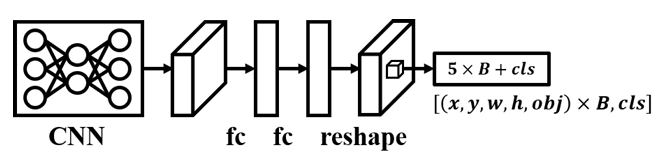
\includegraphics[width=\linewidth]{images/013Methods/yolov1_arch.png}
    \caption{v1}
    \label{subfig_yolov1}
  \end{subfigure}
  \hfill
  \begin{subfigure}{0.32\textwidth}
    \centering
    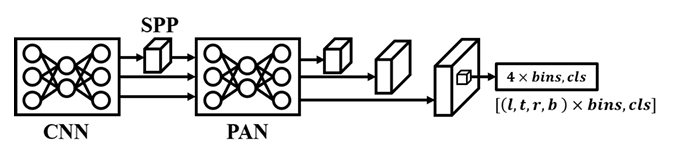
\includegraphics[width=\linewidth]{images/013Methods/yolov8_arch.png}
    \caption{v8}
    \label{subfig_yolov8}
  \end{subfigure}
  \hfill
  \begin{subfigure}{0.32\textwidth}
    \centering
    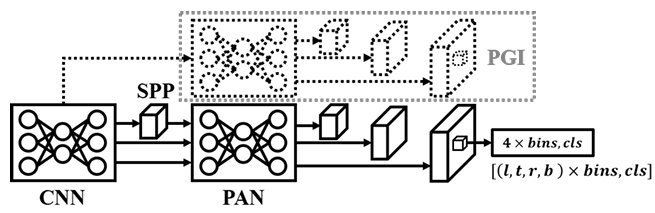
\includegraphics[width=\linewidth]{images/013Methods/yolov9_arch.png}
    \caption{v9}
    \label{subfig_yolov9}
  \end{subfigure}
  
  \caption{Different YOLO Architectures \cite{Wang2024_yolo_review}}
\end{figure}




The development of \acrshort{YOLO} across the various versions shows significant progress. While \acrshort{YOLO}v1 (see Fig. \ref{subfig_yolov1}) was able to save a large number of parameters and computational effort using the One-Stage method by generating predictions using the \acrshort{FCL} in the second layer, \acrshort{YOLO}v8 (see Fig. \ref{subfig_yolov8}) builds on \acrshort{YOLO}v5 and integrates numerous optimisations \cite{Wang2024_yolo_review}. These include the \acrfull{ELAN} integration from \acrshort{YOLO}v7, which has been extended by an additional residual connection, while the decoder is based on \acrshort{YOLO}v6 and remains unchanged. This version also shows an improvement in training performance of about 30\% and enables various downstream tasks such as segmentation, instance segmentation, pose estimation, and multiple object tracking. Finally, \acrshort{YOLO}v9 (see Fig. \ref{subfig_yolov9}) integrates \acrshort{PGI} to prevent important information from being lost at the superficial network level. \acrshort{PGI} ensures more robust performance by retaining the original information as deeply as possible \cite{Wang2024_yolo_review}.

The key strengths of \acrshort{YOLO}v9 lie in its high processing speed and precise object detection, which enable efficient analysis of large data sets.
 
The variants \acrshort{YOLO}v9u and \acrshort{YOLO}v9e differ primarily in terms of the label format used. \acrshort{YOLO}v9e uses a normalised coordinate system:

\hypertarget{eq:yolov9}{}
\begin{equation}
x_\text{norm} = \frac{x_\text{pixel}}{w_\text{image}},\;\;
y_\text{norm} = \frac{y_\text{pixel}}{h_\text{image}},\;\;
w_\text{norm} = \frac{w_\text{box}}{w_\text{image}},\;\;
h_\text{norm} = \frac{h_\text{box}}{h_\text{image}}
\end{equation}
\label{Eq:yolov9}

\hypertarget{eq:yolov9u}{}
In contrast, \acrshort{YOLO}v9u utilises a polygon format.
\begin{equation}
(\text{class\_index},\ x_1, y_1, x_2, y_2, x_3, y_3, x_4, y_4).
\end{equation}



\subsection{YOLOv9u by Wong Kin Yiu}
\label{subsec:yolov9u}

The implementation of \acrshort{YOLO}v9u is based on version \acrshort{YOLO}v8.1.23 \cite{yolo_v9u_github} in order to extend the original \acrshort{YOLO}v9 version with various downstream tasks. These include instance segmentation, oriented object detection, pose estimation, image classification, and transformer-based object detection \cite{wang2024}, whereby a \textit{Detect} layer is integrated with \acrshort{YOLO}v8 as the basis, enabling the prediction of oriented \acrshort{BB}. In this work, \acrshort{YOLO}v9u is used, as it is available as an open-source variant and the underlying methodology has been documented in the published paper \cite{wang2024_sapkota}. The \acrshort{YOLO}v9e model is provided by Ultralytics, but without an accompanying scientific publication, so its structure and methodological basis are not comprehensively documented \cite{ultralyics_2023}.
 



\subsection{YOLOv9e by Ultralytics}
\label{subsec:yolov9e}

The \acrshort{YOLO}v9 model series from Ultralytics comprises several variants that differ in terms of model size, accuracy and computational complexity \cite{ultralyics_yolov9}. All variants integrate the \acrshort{PGI} and \acrshort{GELAN} architectures developed by \citeauthor{wang2024_sapkota} \cite{wang2024_sapkota} and also support the processing of \acrshort{abb}. The range extends from the compact \acrshort{YOLO}v9t variant with an input image size of $640 \times 640$ pixels, 2 million parameters and 7.7 \acrshortpl{GFLOP}, to the most powerful \acrshort{YOLO}v9e variant with 58.1 million parameters and 192.5 \acrshortpl{GFLOP} (see Table~\ref{tab:yolov9-models}).

Due to the highest accuracy achieved (\acrshort{mAP}@0.5-0.95 = 55.6) and the highest computing capacity, the \acrshort{YOLO}v9e model was used for all experiments with axis-aligned bounding boxes. This variant was chosen with the aim of ensuring maximum detection performance during the evaluation. In addition, this version is used because it supports the processing of \acrlong{abb}.




\begin{table}[h]
\centering
\begin{tabular}{l|c|c|c|c|c} % keine äußeren vertikalen Linien
\textbf{Model} & \textbf{Image Size} & \textbf{mAP$_{\text{val}}$ 50--95} & \textbf{mAP$_{\text{val}}$ 50} & \textbf{Parameters (M)} & \textbf{FLOPs (B)} \\
\hline
YOLOv9t & 640 & 38.3 & 53.1 & 2.0 & 7.7 \\
YOLOv9s & 640 & 46.8 & 63.4 & 7.2 & 26.7 \\
YOLOv9m & 640 & 51.4 & 68.1 & 20.1 & 76.8 \\
YOLOv9c & 640 & 53.0 & 70.2 & 25.5 & 102.8 \\
YOLOv9e & 640 & 55.6 & 72.8 & 58.1 & 192.5 \\
\end{tabular}
\caption[Comparison of YOLOv9 model variants]{Comparison of YOLOv9 model variants in terms of accuracy and computational complexity at an input resolution of 640$\times$640 pixels. \cite{ultralyics_yolov9,wang2024_sapkota}}
\label{tab:yolov9-models}
\end{table}



%##########################################################################
%##########################################################################
%##########################################################################
%##########################################################################
%##########################################################################
%##########################################################################
%##########################################################################
%##########################################################################


\section{Programming Environment}
The programming language used is Python. The scripts for \acrlong{HPC} \acrshort{PALMA} were written in Bash.

\subsection{Python Packages}
Various Python packages were used for implementation, which are briefly described below.
 
\subsubsection{Computer Vision 2}
Part of the ‘Open Source Computer Vision’ library is \Acrfull{CV2} \cite{opencv_about}. The current version 4.12.0 was released on 9 July 2025 \cite{opencv_release}. \\
The library offers algorithms and functions for image and video processing, which are mainly used in this work to combine the different channels into new images. It should be noted that \acrshort{CV2} stores images as BGR (blue, green, red) colour combinations, which can lead to false colour representations of some images that are displayed in RGB (such as Fig. \ref{fig:perm_exp_example_pics}).
\subsubsection{Numpy}
Another open-source project is NumPy, which was founded in 2005 to implement numerical operations in Python \cite{numpy_about}. The current version is 2.3.0 and was released on 7 June 2025 \cite{numpy_main_web}. \\
With the help of this library, a random distribution of the image data across the folds can be achieved by subjecting the imported image list to a random permutation. In addition, the library provides functions that can be used to calculate and rescale the \acrshort{NDVI} channel and transform the bounding box coordinates into the format required for the \acrshort{YOLO} framework. It also enables the conversion of axis-aligned bounding boxes into oriented bounding boxes and the calculation of the area of both bounding box types.
\subsubsection{Scipy}
SciPy version 1.16.0 was released on 22 June 2025 \cite{scipy-main}. This library provides algorithms for scientific calculations in Python \cite{scipy-main}. The subfunction ‘ConvexHull’ is used to calculate the area of oriented bounding boxes.
\subsection{Additional Python packages for data analysis}
The following libraries were used to analyse the models.
\subsubsection*{Matplotlib}
The ‘Matplotlib’ library was released in version 3.10.0 on 23 December 2024 \cite{matplotlib}. In the context of this work, this extension enables data analysis and the output of plots.
\subsubsection*{Seaborn}
‘Seaborn’ was released in version 0.13.2 in January 2024 \cite{seaborn}. The library enables the creation of graphics, such as box plots, for simplified data analysis.
\subsubsection*{pandas}
The ‘pandas’ library is also an open source data analysis and manipulation tool. The current version 2.3.1 was released on 7 July 2025. The library is also used for data analysis in this work \cite{pandas}.

%!TEX root = ../thesis.tex
\chapter{Implementation}
\label{ch:implementation}




\section{Challenges Preprocessing}
Several technical challenges arose during the processing of the VEDAI dataset.
First, the existing labels had to be converted to the \acrshort{YOLO}v9-\acrshort{obb} format to be compatible with the selected model.
It was found that a small subset of the data (7 out of 3,757 cases) had coordinate values outside the permissible range (i.e. less than 0 (see Fig. \ref{fig:smaller0}) or greater than 1 (see Fig. \ref{fig:higher1})). 
This problem was resolved by using exception handling and rounding the values to the valid value range.
 

\begin{figure}[h]
    \centering
    \begin{subfigure}[b]{0.45\textwidth}
        \centering
        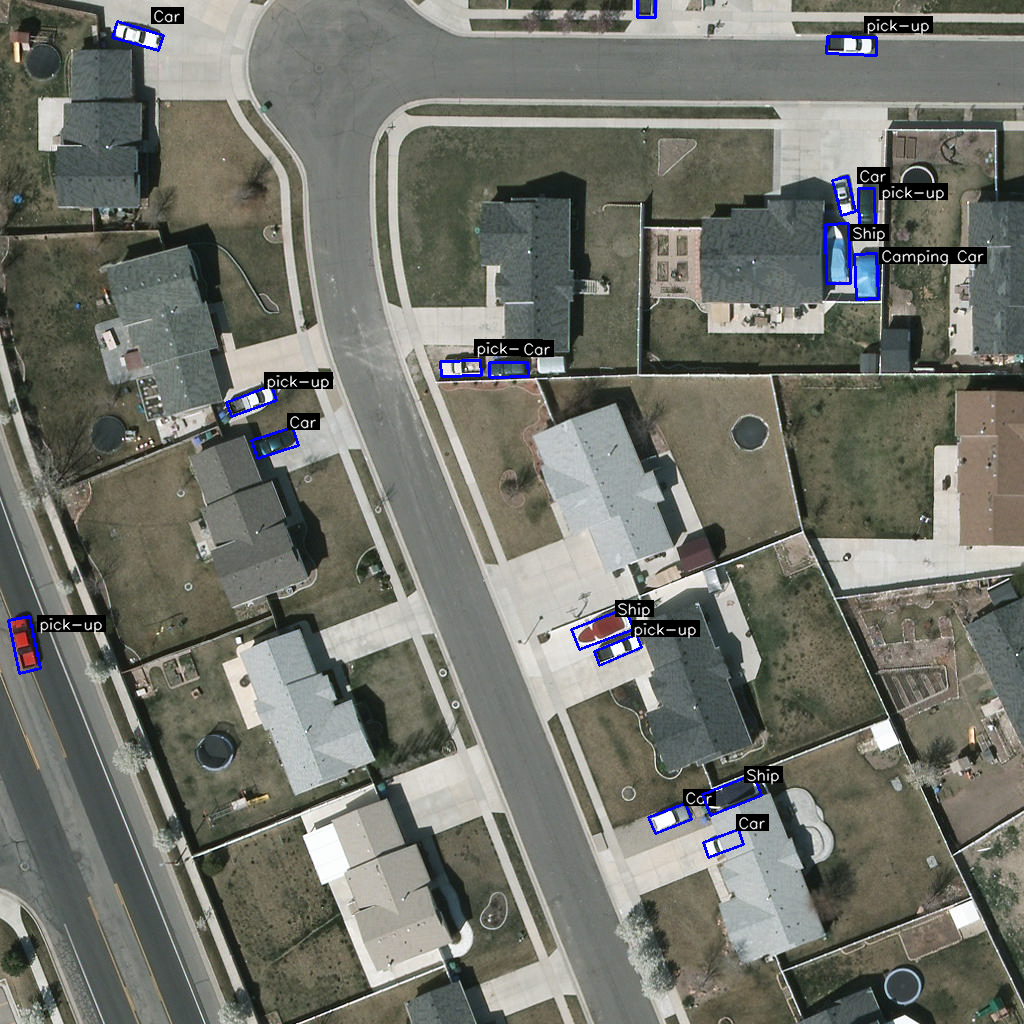
\includegraphics[trim={600pt 1000pt 350pt 0pt},clip,width=\textwidth]{images/bb_smaller0.png}
        \caption{Two Coordinate out of range and smaller 0}
        \label{fig:smaller0}
    \end{subfigure}
    \hfill
    \begin{subfigure}[b]{0.45\textwidth}
        \centering
        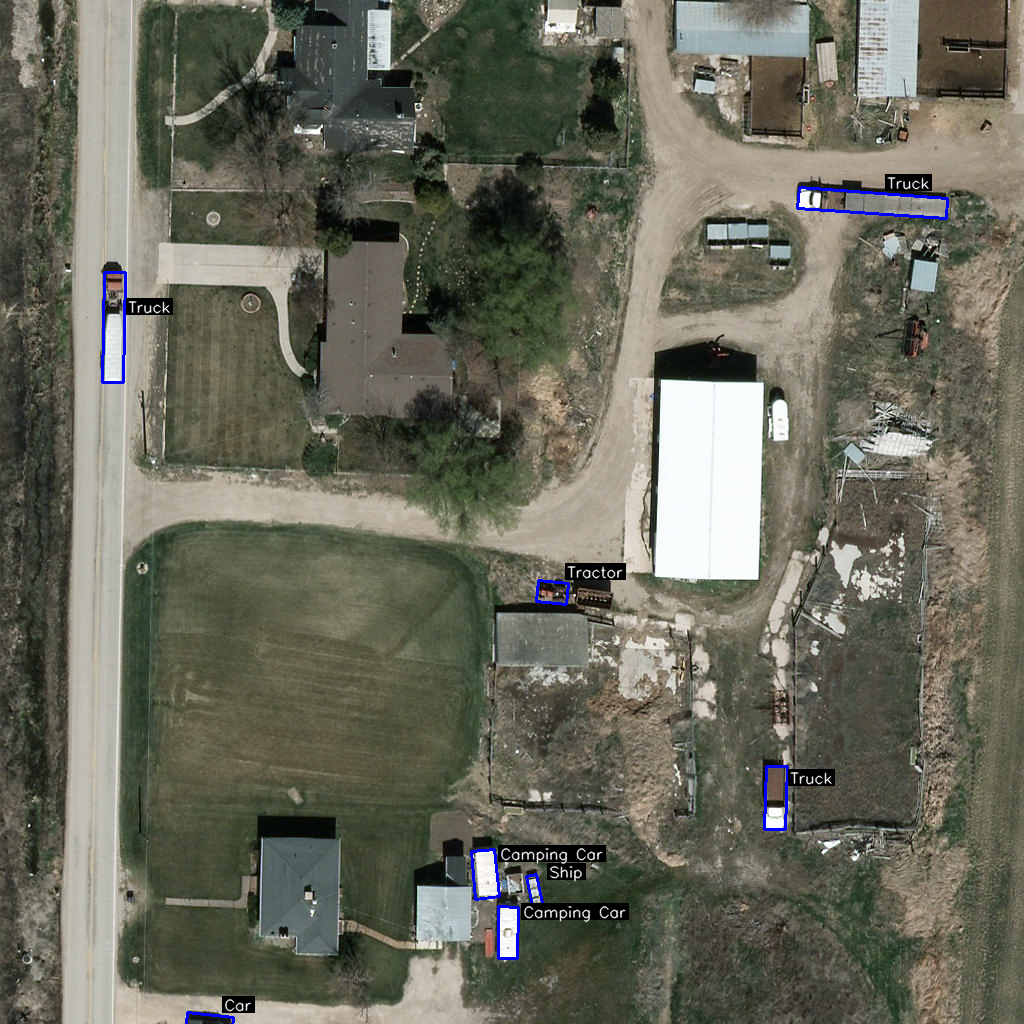
\includegraphics[trim={180pt 0pt 750pt 993pt},clip,width=\textwidth]{images/bb_higher1.png}
        \caption{Two Coordinates out ouf range and higher 1}
        \label{fig:higher1}
    \end{subfigure}
    \caption[Example for label coordinates outside of the image]{Example for label coordinates outside of the image (for full-sized Image see \ref{fig:example_coords_ooR_fs})}
    \label{fig:example_coords_ooR}
\end{figure}







\section{6-Fold-Cross-Validation}
\label{sec_5Fold_CV}


To ensure the robustness of the results and enable a sound comparison of different models, 6-fold cross-validation was used in this study. In particular, emphasis was placed on not only performing the evaluation on a partial data set, but also on dividing the data multiple times to minimise fluctuations caused by different training and validation divisions.

In contrast to the folds provided by \citeauthor{Razakarivony2015} \cite{Razakarivony2015}, whose compilation contains identical images in both the training and validation sets, separate, disjoint folds were generated for this work. The latter ensure that there is no overlap between training and validation data, thus eliminating the risk of distorted training results due to overfitting. The exact methodology of fold creation is described in Chapter \ref{subsec:Fold_creation}.

The data was divided into six folds (0-5): Five folds (folds 0 to 4) were used for training and validation, while fold 5 was reserved exclusively for final testing purposes. This ensured that the final evaluation was carried out on previously unseen, neutral data.

Special attention was paid to ensuring a homogeneous distribution of objects and object classes across all folds. Each fold comprises between 207 and 221 images, including three to seven pure background images without objects. This enabled a balanced and representative evaluation of the models with regard to all occurring classes. The resulting class and image distribution per fold is shown in Table~\ref{tab:fold_distribution}.

Overall, this procedure contributes to the high validity of the experimental results and allows reliable conclusions to be drawn about the effects of the additional channels in the models used.


\begin{table}[h!]
\centering
\begin{tabular}{lcccccc}
\textbf{Class/Fold} & \textit{0} & \textit{1} & \textit{2} & \textit{3} & \textit{4} & \textit{5} \\
\hline
\textit{Car}              & 229 & 239 & 226 & 225 & 240 & 225 \\
\textit{Truck}            & 51  & 57  & 50  & 49  & 51  & 50  \\
\textit{Ship}             & 30  & 28  & 29  & 30  & 27  & 27  \\
\textit{Tractor}          & 30  & 32  & 33  & 30  & 31  & 30  \\
\textit{Camping car}      & 65  & 72  & 64  & 69  & 64  & 63  \\
\textit{Van}              & 18  & 17  & 17  & 17  & 16  & 16  \\
\textit{Vehicle}          & 34  & 37  & 34  & 34  & 39  & 33  \\
\textit{Pick-Up}          & 164 & 161 & 157 & 160 & 159 & 157 \\
\textit{Plane}            & 4   & 11  & 4   & 18  & 4   & 7   \\
\textit{Quantity Images}  & 206 & 214 & 221 & 211 & 207 & 209 \\
\textit{Background Images}& 7   & 3   & 3   & 3   & 3   & 3   \\
\hline
\end{tabular}
\caption{Class distribution across folds.}
\label{tab:fold_distribution}
\end{table}



\section{High-Performance-Cluster PALMA}

The \acrfull{HPC} \Acrshort{PALMA} at the University of Münster was used to train the models. An isolated Python environment (UV \cite{palma_uv}) was used as the working environment. The training processes were executed using self-developed Bash scripts, which were distributed across different \acrshort{GPU} nodes of the cluster (including HGX nodes) to enable efficient parallelisation of the training.

PALMA (abbreviation for ‘\Acrlong{PALMA}’) is provided by the \Acrfull{CIT} at the University of Münster, based on hardware from MEGWARE \cite{palma_spec}, and has the technical specifications listed in Table \ref{tab:Spec_Palma} \cite{palma_spec}:




\begin{table}[h!]
\centering
\begin{tabular}{ll}
\multicolumn{2}{c}{\textbf{Palma Specifications}} \\ \hline
\textbf{Total number of \acrshort{CPU} cores} & 16,272 \\
\textbf{Memory} & 77,568\,\acrshort{GB} \\
\textbf{Number of compute nodes} & 444 \\
\textbf{Processor} & Intel Xeon Gold 6140 (18~cores, 2.30\,\acrshort{GHz}, Skylake architecture) \\
\textbf{Network interconnect} & 100\,\acrshort{GHz}/s Intel Omni-Path \\
\textbf{Storage system} & \acrshort{GPFS} with a total capacity of 2.4\,\acrshort{PB} \\
\textbf{Linpack performance} & \textit{R\textsubscript{max}} = 800\,\acrshort{TFLOP}/s; \textit{R\textsubscript{peak}} = 1,277\,\acrshort{TFLOP}/s \\
\textbf{Operating system} & Rocky Linux 9 \\
\hline
\end{tabular}
\caption{System overview PALMA}
\label{tab:Spec_Palma}
\end{table}

The cluster's high computing power and storage capacity made it possible to process even complex training processes with large amounts of high-resolution image data efficiently and quickly.



\section{Bash Scripts}

Several Bash scripts were developed for training the models, which were designed for the high-performance computer \acrshort{PALMA}. The training runs were primarily carried out using \acrshort{SLURM} job arrays, with each fold of a permutation being assigned to a separate job. Thus, a model always corresponded to a fold within a specific permutation.  

The decision between \acrlongpl{abb} and \acrlongpl{obb} was made using the same training parameters as in the permutation experiments (see Table~\ref{tab:hyperparameters}), but with different models: \acrshort{YOLO}v9e for \acrshort{abb} and \acrshort{YOLO}v9u for \acrshort{obb}, as only these variants support the corresponding bounding box formats. In this case, no pre-trained model was used; instead, training was carried out \textit{from scratch}.
  
The permutation experiments were then carried out. The hyperparameters listed in Table~\ref{tab:hyperparameters} were used consistently. The image resolution was 1024~$\times$~1024 pixels, the training duration was 500 epochs, and early termination was disabled by setting the \texttt{patience} value to 0 to ensure consistent comparability. The basis was a model pre-trained on the \acrshort{DOTA} dataset, using the \acrshort{YOLO}v9u architecture (see section~\ref{subsec:yolov9u}) throughout.
  
For the ablation studies, however, the use of a pre-trained model was dispensed with, while all other training parameters remained unchanged.  

After completion of the training, the model with the best validation performance was selected and then applied to the corresponding test fold. In both cases, the evaluation was carried out in a single run to ensure consistent and comparable results.
    



\begin{table}[htbp]
\centering

\begin{tabular}{ll}
\hline
\textbf{Hyperparameter} & \textbf{Value / Description} \\
\hline
Task & Oriented Bounding Box (OBB) \\
Mode & Training \\
Model & YOLOv9u, pretrained on \acrshort{DOTA} \\
Dataset & \acrshort{VEDAI}  \\
Epochs & 500 \\
Batch size & 4 \\
Image size & 1024 × 1024 px \\
Early stopping (patience) & 0 (disabled) \\
Optimizer & Auto \\
Initial learning rate ($lr_0$) & 0.01 \\
Momentum & 0.937 \\
Weight decay & 0.0005 \\
Warmup epochs & 3 \\
Data augmentation & FlipLR 0.5, Mosaic 1.0, Erasing 0.4, AutoAugment randaugment \\
Device & GPUs 0,1,2,3 \\
Workers & 8 \\
Save directory & \texttt{/scratch/tmp/t\_liet02/cross\_validation/rgb/fold4} \\
\hline
\end{tabular}
\caption{Key training hyperparameters at the \acrshort{RGB} Permutation (Fold 4)}
\label{tab:hyperparameters}
\end{table}



